\documentclass[border=16pt]{standalone}
\usepackage[T1]{fontenc}
\usepackage{amsmath}
\usepackage{tikz}
\usetikzlibrary{positioning,arrows.meta,fit,backgrounds,calc,decorations.pathreplacing}

\definecolor{clsBlue}{HTML}{2C5AA0}
\definecolor{clsBg}{HTML}{EAF1FA}
\definecolor{ownGreen}{HTML}{1F7A5A}
\definecolor{ownBg}{HTML}{E4F3EC}
\definecolor{viewOr}{HTML}{C4600A}
\definecolor{viewBg}{HTML}{FCEBD7}
\definecolor{hl}{HTML}{FFD35C}
\definecolor{ink}{HTML}{333333}

\def\cw{0.86}\def\ch{0.66}\def\pitch{1.02}\def\cellsx{7.6}

\begin{document}
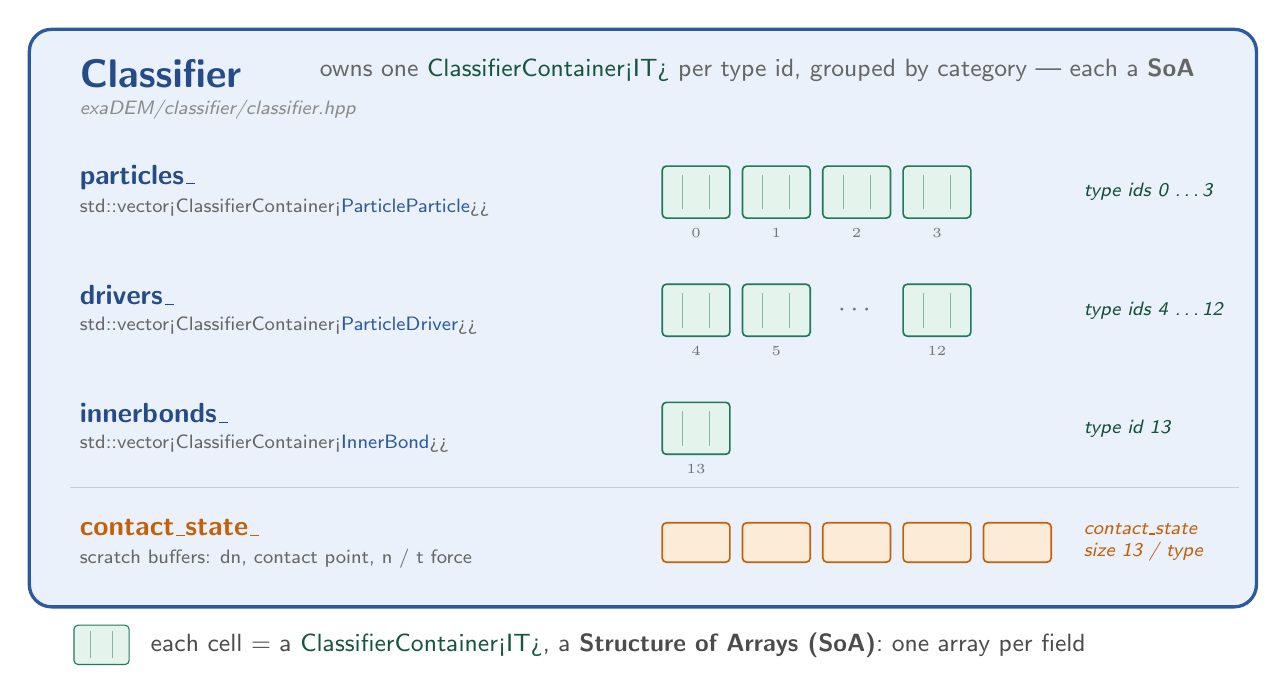
\begin{tikzpicture}[
  font=\sffamily,
  >=Stealth,
  memname/.style={font=\sffamily\bfseries, text=clsBlue!85!black},
  typ/.style={font=\sffamily\scriptsize, text=black!60},
  sizetag/.style={font=\sffamily\scriptsize\itshape, text=ownGreen!65!black, anchor=west},
  bigbox/.style={rounded corners=8pt, line width=1.2pt},
  callout/.style={rounded corners=5pt, line width=0.9pt, align=left, font=\sffamily\small},
]

% ---------- container cell (a ClassifierContainer<IT>, SoA hint) ----------
\newcommand{\cc}[4]{% x y indexlabel hl
  \ifnum#4=1 \def\ccfill{hl}\else \def\ccfill{ownBg}\fi
  \node[draw=ownGreen,line width=0.6pt,fill=\ccfill,rounded corners=1.5pt,
        minimum width=\cw cm,minimum height=\ch cm] at (#1,#2){};
  \draw[ownGreen!55,line width=0.35pt] (#1-0.17,#2-0.22)--(#1-0.17,#2+0.22);
  \draw[ownGreen!55,line width=0.35pt] (#1+0.17,#2-0.22)--(#1+0.17,#2+0.22);
  \node[font=\tiny,text=black!55] at (#1,#2-0.52){#3};}
\newcommand{\ellip}[2]{\node[text=black!55] at (#1,#2){$\cdots$};}

% =====================================================================
% TITLE
% =====================================================================
\node[memname, font=\sffamily\Large\bfseries, anchor=west] at (-0.35,1.5){Classifier};
\node[font=\sffamily\small, text=black!60, anchor=west] at (2.7,1.55)
     {owns one \textcolor{ownGreen!70!black}{ClassifierContainer<IT>} per type id, grouped by category --- each a \textbf{SoA}};
\node[font=\sffamily\scriptsize\itshape, text=black!45, anchor=west] at (-0.35,1.05)
     {exaDEM/classifier/classifier.hpp};

% =====================================================================
% ROW 1 : particles_  (13 containers)
% =====================================================================
\def\Ry{0}
\node[memname, anchor=west]  at (-0.35,\Ry+0.19){particles\_};
\node[typ, anchor=west]   at (-0.35,\Ry-0.2){std::vector<ClassifierContainer<\textcolor{clsBlue}{ParticleParticle}>>};
\cc{\cellsx}{\Ry}{0}{0}
\cc{\cellsx+\pitch}{\Ry}{1}{0}
\cc{\cellsx+2*\pitch}{\Ry}{2}{0}
\cc{\cellsx+3*\pitch}{\Ry}{3}{0}
\node[sizetag] at (12.4,\Ry){type ids 0 \dots 3};

% =====================================================================
% ROW 2 : drivers_
% =====================================================================
\def\Sy{-1.5}
\node[memname, anchor=west]  at (-0.35,\Sy+0.19){drivers\_};
\node[typ, anchor=west]   at (-0.35,\Sy-0.2){std::vector<ClassifierContainer<\textcolor{clsBlue}{ParticleDriver}>>};
\cc{\cellsx}{\Sy}{4}{0}
\cc{\cellsx+\pitch}{\Sy}{5}{0}
\ellip{\cellsx+2*\pitch}{\Sy}
\cc{\cellsx+3*\pitch}{\Sy}{12}{0}
\node[sizetag] at (12.4,\Sy){type ids 4 \dots 12};

% =====================================================================
% ROW 3 : innerbonds_  (1 container)
% =====================================================================
\def\Ty{-3.0}
\node[memname, anchor=west]  at (-0.35,\Ty+0.19){innerbonds\_};
\node[typ, anchor=west]   at (-0.35,\Ty-0.2){std::vector<ClassifierContainer<\textcolor{clsBlue}{InnerBond}>>};
\cc{\cellsx}{\Ty}{13}{0}
\node[sizetag] at (12.4,\Ty){type id 13};

% divider
\draw[black!20,line width=0.6pt] (-0.35,-3.75)--(14.5,-3.75);

% =====================================================================
% ROW 4 : contact_state_  (per-type scratch buffers, NOT persisted)
% =====================================================================
\def\Cy{-4.45}
\node[memname, text=viewOr, anchor=west] at (-0.35,\Cy+0.19){contact\_state\_};
\node[typ, anchor=west] at (-0.35,\Cy-0.2){scratch buffers: dn, contact point, n / t force};
\foreach \k in {0,1,2,3,4}{
  \node[draw=viewOr,line width=0.6pt,fill=viewBg,rounded corners=1.5pt,
        minimum width=\cw cm,minimum height=0.5cm] at (\cellsx+\k*\pitch,\Cy){};}
\node[sizetag, text=viewOr, align=left] at (12.4,\Cy){contact\_state\\ size 13 / type};

% =====================================================================
% CLASSIFIER BOX (drawn behind)
% =====================================================================
\begin{scope}[on background layer]
  \node[draw=clsBlue, bigbox, fill=clsBg, fit={(-0.75,1.95) (14.6,-5.15)}] (clsbox){};
\end{scope}

% =====================================================================
% LEGEND : cells are SoA containers
% =====================================================================
\node[draw=ownGreen,fill=ownBg,rounded corners=1.5pt,minimum width=0.7cm,minimum height=0.5cm] at (0.05,-5.75){};
\draw[ownGreen!55,line width=0.35pt] (0.05-0.14,-5.75-0.17)--(0.05-0.14,-5.75+0.17);
\draw[ownGreen!55,line width=0.35pt] (0.05+0.14,-5.75-0.17)--(0.05+0.14,-5.75+0.17);
\node[anchor=west, font=\sffamily\small, text=black!70] at (0.55,-5.75)
  {each cell = a \textcolor{ownGreen!70!black}{ClassifierContainer<IT>}, a \textbf{Structure of Arrays (SoA)}: one array per field};

\end{tikzpicture}
\end{document}
